%%%%%%%%%%%%%%%%%%%%%%%%%%%%%%%%%%%%%%%%%%%%%%%%%%%%%%%%%%%
% Conclusiones teoría de la aproximación 
%%%%%%%%%%%%%%%%%%%%%%%%%%%%%%%%%%%%%%%%%%%%%%%%%%%%%%%%%%%
\section{Conclusiones teoría de la aproximación} 
\label{ch03:conclusiones-teoria-aproximacion}
Acabamos de probar en \ref{ch:TeoremaStoneWeiertrass} que cualquier función 
continua es aproximable uniformemente con polinomios en un compacto. 
Sin embargo este enfoque tiene los siguientes problemas: 

\begin{enumerate}
    \item La prueba obtenida no nos permite 
    una forma constructiva sencilla de obtener el polinomio. 
    \item Aproximando con polinomios se corre el riesgo de que fuera de la muestra 
    el error sea demasiado grande. Como muestra de ello damos un ejemplo patológico 
    reflejado en la figura \ref{fig:aproximacion-lagrage}; se pretende aproximar 
    la función $f:[-3,3] \longrightarrow \R$ definida como
    \begin{equation*}
        f(x)= \left\{ \begin{array}{lcc}
            e^{-x} + 4 &   si  & x \leq 1 \\
            \\ \log{x} &  si  & x > 1
            \end{array}
  \right.
    \end{equation*}
    usando el método de interpolación de Lagrange; en este caso el error tiende a 
    infinito conforme aumenta el número de nodos. \footnote{Puede encontrar la implementación
    del código que genera las gráficas en nuestro repositorio 
    \url{https://github.com/BlancaCC/TFG-Estudio-de-las-redes-neuronales}, 
    en el fichero \texttt{Lagrange.ipynb} que se encuentra  en el directorio de teoría de la aproximación de la memoria. } 

    El problema que evidencia este caso patológico es el tratar de abarcar todo el dominio 
con un mismo polinomio ¿y si en lugar de eso se hicieran aproximaciones 
en una partición concreta del dominio? El resultado sería una función definida a trozos.   
La cuestión es que esta aproximación sería difícil de implementar de manera eficiente;
sin embargo, es el germen y el enfoque de las \textit{funciones de activación}. 

    \item Y otra cuestión, de corte físico o  filosófico ¿son todos los fenómenos observables continuos? 
    Sería extraño que así fueran, lo que evidencia la necesidad de formular una teoría más general. 
\end{enumerate}


De todas formas no abandonaremos del todo esta teoría; porque como ya veremos, el 
teorema de Stone Weierstrass  \ref{ch:TeoremaStoneWeiertrass} jugará 
un papel fundamental en el diseño y demostración de
 las redes neuronales como aproximadores universales,
 ya que nos brinda los requisitos mínimo que debe de tener un conjunto para ser capaz de aproximar cualquier función continua.

%\newpage

\begin{figure}[H]
    \centering
    \begin{subfigure}[b]{0.475\textwidth}
        \centering
        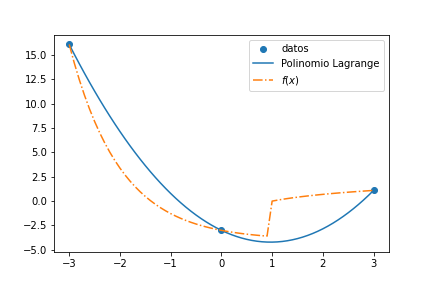
\includegraphics[width=\textwidth]{metodo-lagrange/lagrange-3-datos.png}
        \caption[Network2]%
        {{\small Polinomio de Lagrange utilizando 3 datos}}    
    \end{subfigure}
    \hfill
    \begin{subfigure}[b]{0.475\textwidth}  
        \centering 
        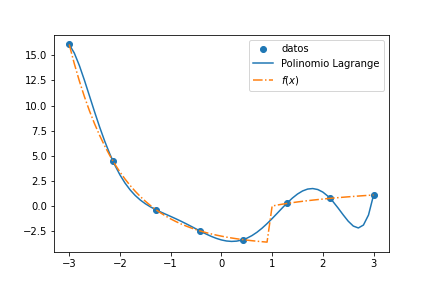
\includegraphics[width=\textwidth]{metodo-lagrange/lagrange-8-datos.png}
        \caption[]%
        {{\small Polinomio de Lagrange utilizando 8 datos}}    
    \end{subfigure}
    \vskip\baselineskip
    \begin{subfigure}[b]{0.475\textwidth}   
        \centering 
        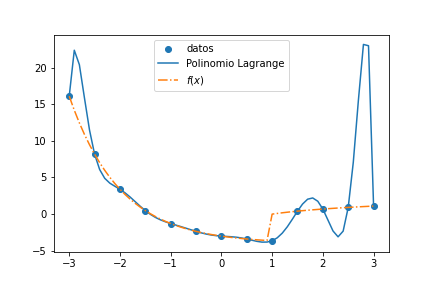
\includegraphics[width=\textwidth]{metodo-lagrange/lagrange-13-datos.png}
        \caption[]%
        {{\small Polinomio de Lagrange utilizando 13 datos}}    
    \end{subfigure}
    \hfill
    \begin{subfigure}[b]{0.475\textwidth}   
        \centering 
        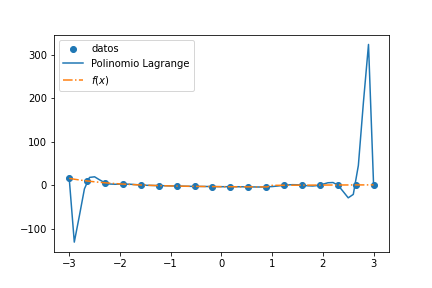
\includegraphics[width=\textwidth]{metodo-lagrange/lagrange-18-datos.png}
        \caption[]%
        {{\small Polinomio de Lagrange utilizando 18 datos}}    
    \end{subfigure}
    \caption{Ejemplo de aproximación de la función $f(x)$ a partir de los polinomios de Lagrange.} 
    \label{fig:aproximacion-lagrage}
\end{figure}

